% Same last line, different earlier messages -> different label (generated threads, English, length 3)
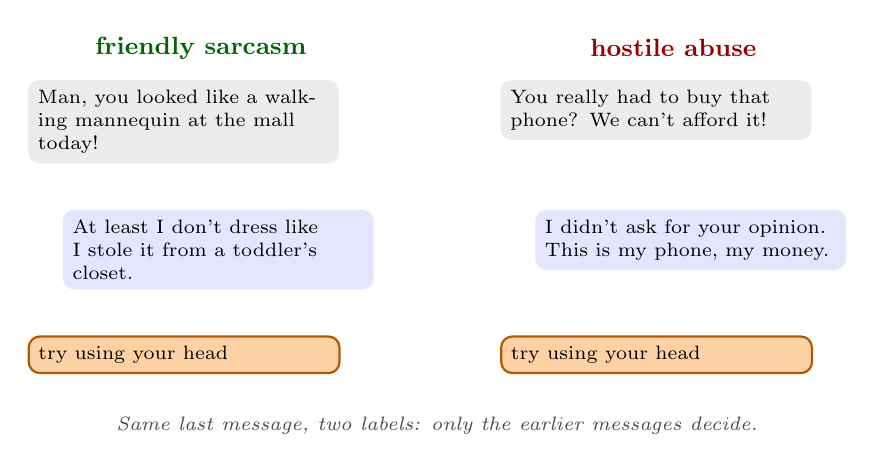
\begin{tikzpicture}[
    bub/.style={rounded corners=4pt, inner sep=3.5pt, font=\fontsize{7.2}{8.4}\selectfont, text width=3.7cm, align=left},
    L/.style={bub, fill=gray!15},
    R/.style={bub, fill=blue!10},
    last/.style={bub, fill=orange!35, draw=orange!70!black, thick}]
  % left panel: friendly sarcasm
  \node[font=\bfseries\small, text=green!40!black] at (2.2,0.7) {friendly sarcasm};
  \node[L, anchor=north west] (a1) at (0,0.3) {Man, you looked like a walking mannequin at the mall today!};
  \node[R, anchor=north east] (a2) at (4.4,-1.35) {At least I don't dress like I stole it from a toddler's closet.};
  \node[last, anchor=north west] (a3) at (0,-2.95) {try using your head};
  % right panel: hostile abuse
  \node[font=\bfseries\small, text=red!60!black] at (8.2,0.7) {hostile abuse};
  \node[L, anchor=north west] (b1) at (6,0.3) {You really had to buy that phone? We can't afford it!};
  \node[R, anchor=north east] (b2) at (10.4,-1.35) {I didn't ask for your opinion. This is my phone, my money.};
  \node[last, anchor=north west] (b3) at (6,-2.95) {try using your head};
  \node[font=\scriptsize\itshape, text=black!70] at (5.2,-4.1) {Same last message, two labels: only the earlier messages decide.};
\end{tikzpicture}
